%% Working paper in ICML 2026 format (not for submission).
%% Every number in this file comes from the summaries listed in REPRODUCIBILITY.md:
%% out/online_200k_summary.txt (Study 1), out/alpha_200k_summary.txt and
%% out/alpha_200k_pooled_and_diag.txt (Study 2), out/replication_200k_summary.txt and
%% out/replication_200k_pooled.txt (Study 3), out/burnin_200k_summary.txt and
%% out/burnin_200k_pooled.txt (Study 4), out/rate_200k_summary.txt and
%% out/rate_200k_pooled.txt (Study 5), dev_checks/out_*.txt (checks).
\documentclass{article}

\usepackage{microtype}
\usepackage{graphicx}
\usepackage{booktabs}
\usepackage{hyperref}
\newcommand{\theHalgorithm}{\arabic{algorithm}}
\usepackage{icml2026}
\usepackage{amsmath}
\usepackage{amssymb}
\usepackage{mathtools}
\usepackage{amsthm}
\usepackage[capitalize,noabbrev]{cleveref}
\usepackage{algorithm}
\usepackage{algorithmic}

\newcommand{\dS}{\Delta s}
\newcommand{\one}{\mathbb{1}}

\icmltitlerunning{Generative Replay from a Single Self-Organizing Map}

\begin{document}

\twocolumn[
  \icmltitle{Generative Replay from a Single Self-Organizing Map:\\
    How Units Summarise and Generate Experience}

  \begin{icmlauthorlist}
    \icmlauthor{Anonymous Authors}{anon}
  \end{icmlauthorlist}

  \icmlaffiliation{anon}{Working draft, not for submission}
  \icmlcorrespondingauthor{Anonymous}{anon@anon}

  \icmlkeywords{Self-Organizing Maps, Experience Replay, Generative Replay, Deep Q-Learning, Memory-Bounded Reinforcement Learning}

  \vskip 0.3in
]

\printAffiliationsAndNotice{}

\begin{abstract}
Replay buffers let value-based agents reuse experience, but they store raw
transitions and must discard them when memory is bounded. We study a replay
memory that stores none: a single Self-Organizing Map learns online from the
agent's stream, each unit keeps running statistics of the transitions it
represents, and every training minibatch is generated from those statistics.
Through five pre-registered studies with an online Deep Q-Network on
CartPole, we isolate which design choices matter. How each unit summarises
its transitions, and in particular how it generates episode endings, matters
far more than how transitions are assigned to units. With exact per-unit
averages and endings drawn at each unit's recorded rate, the map exceeds a
first-in-first-out buffer of real transitions with the same memory over
200\,000 steps, and it is clearly better than reservoir and
ending-preserving buffers. The averaging rate trades a fast start against
late performance.
\end{abstract}

\section{Introduction}
\label{sec:intro}

Experience replay \citep{lin1992self} is central to value-based deep
reinforcement learning (RL): a Deep Q-Network \citep[DQN;][]{mnih2015human}
learns from minibatches drawn from a buffer of past transitions, which reuses
data and breaks the correlation of consecutive steps. The buffer stores raw
transitions, so under a memory bound it must decide what to keep. A
first-in-first-out (FIFO) buffer keeps the most recent transitions, reservoir
sampling keeps a uniform sample of everything seen
\citep{vitter1985random,isele2018selective}, and other rules favour rare or
informative transitions \citep{schaul2016prioritized,hayes2019memory}.

Generative replay replaces stored data with a model that produces training
data on demand \citep{shin2017continual}. A Self-Organizing Map
\citep[SOM;][]{kohonen1982self,kohonen2001som} is a natural model for an
online, memory-bounded agent. It learns from one sample at a time, its size
is fixed in advance, and each unit summarises one region of the data. SOMs
have stored and transferred knowledge in RL \citep{karimpanal2019som} and
have served as compact replay memories whose nodes and edges are replayed
\citep{hafez2023map}; uncertainty has been proposed as a signal for what a
replay memory should hold \citep{rajakrishnan2026uncertainty}.

A SOM replay memory involves many design choices: how transitions are
assigned to units, how each unit summarises the transitions it receives,
which units generate, and how the discrete parts of a transition (the action
and the episode ending) are produced. This paper studies these choices in the
simplest setting, a single map over whole transitions that generates
independent transitions as the only replay memory of an online DQN agent. Our
contributions are:

\begin{itemize}
\item A SOM replay memory with a structured, standardised distance over
  $[s, a, r, \dS, d]$, per-unit Gaussian statistics and explicit memory
  accounting (\cref{sec:method}).
\item Five pre-registered studies, with claims written before each run,
  that separate the effect of the per-unit estimator, the covariance, the
  choice of units and the decoding of episode endings
  (\cref{sec:setup,sec:results}).
\item The finding that the decoding of episode endings and the per-unit
  estimator dominate: with exact averages and endings drawn at each unit's
  recorded rate, the map matched or exceeded a FIFO buffer of the same memory
  over the whole run, while a fast exponential average with rounded endings
  fell behind FIFO late in training.
\end{itemize}

\section{Related Work}
\label{sec:related}

\paragraph{Bounded replay.} Which transitions to keep under a memory bound
has been studied for lifelong and streaming learning: reservoir sampling and
coverage-based selection \citep{isele2018selective}, and memory-efficient
buffers for streaming classification \citep{hayes2019memory}. Prioritised
replay \citep{schaul2016prioritized} changes which stored transitions are
sampled, not which are kept. All of these store raw transitions.

\paragraph{Generative replay.} Deep generative replay
\citep{shin2017continual} trains a generator alongside the learner and
replays its samples to prevent forgetting. Our memory is a generative model
of transitions, but one that learns in a single online pass with a fixed
number of stored numbers.

\paragraph{Self-organizing maps in RL and replay.} \citet{karimpanal2019som}
use SOMs to store and transfer knowledge between tasks. \citet{hafez2023map}
build a growing map of states whose nodes and edges are replayed, reducing
memory while limiting forgetting. \citet{rajakrishnan2026uncertainty} use
uncertainty to drive what a replay memory holds. SOM-based synthetic replay
has also been used for unsupervised continual learning
\citep{thapa2026unsupervised}. We study a single fixed-size map whose units
keep Gaussian statistics of whole transitions, and ask which of its design
choices matter for an online value-based learner.

\section{Method}
\label{sec:method}

\subsection{Setting}
\label{sec:setting}

An agent acts with an $\epsilon$-greedy policy. Each step yields a transition
$(s, a, r, s', d)$ with state $s \in \mathbb{R}^{n}$, discrete action $a$,
reward $r$, next state $s'$ and ending flag $d$. The transition is written to
the replay memory once and not seen again; after each step the agent takes
one gradient step on a minibatch returned by the memory. Memory is counted
in stored numbers: a real transition costs $2n + 3$ of them ($n = 4$ on
CartPole, so 11). The flag $d$ marks only terminal states; a stop at the
environment's time limit is not terminal \citep{pardo2018time}.

\subsection{Transition vector and distance}
\label{sec:distance}

The memory is one SOM with a $10 \times 10$ grid of units. Each transition is
written as
\begin{equation}
  x = [\,s,\; a,\; r,\; \dS,\; d\,], \qquad \dS = s' - s,
  \label{eq:vector}
\end{equation}
which separates where the agent is ($s$) from how the system moves ($\dS$).
The continuous channels $s$, $r$ and $\dS$ are z-scored with a running mean
and standard deviation updated at every step \citep{welford1962note}; $a$
and $d$ stay 0/1. We write $\tilde{x}$ for the standardised vector.

The best-matching unit (BMU) of a transition is the unit whose weight vector
$w$ minimises
\begin{multline}
  D(\tilde{x}, w) = \alpha_s \sum_{i} \beta_i (\tilde{s}_i - w_{s,i})^2
  + \alpha_a \one[a \neq \lfloor w_a \rceil] \\
  + \alpha_r (\tilde{r} - w_r)^2
  + \alpha_{\Delta} \sum_i \gamma_i (\widetilde{\dS}_i - w_{\Delta,i})^2
  + \alpha_d \one[d \neq \lfloor w_d \rceil],
  \label{eq:distance}
\end{multline}
where $\lfloor\cdot\rceil$ rounds to the nearest valid value. Actions and
endings are categorical and are compared by mismatch. We use $\alpha_s = 1$,
$\alpha_a = 0.5$, $\alpha_r = 0$ (CartPole's reward is constant),
$\alpha_\Delta = 1$ and $\alpha_d = 1$. Within the state,
$\beta = [0.5, 0.5, 2.0, 1.5]$ for cart position, cart velocity, pole angle
and pole angular velocity, favouring the variables that predict a fall.
Within the change of state, $\gamma = [0, 0.5, 0, 1.5]$: CartPole's
integrator sets $\Delta x = \tau \dot{x}$ and $\Delta\theta = \tau
\dot{\theta}$, so after standardisation these two channels repeat the
velocities, and weighting them would count the velocities twice.

\paragraph{Map update.} The BMU $c$ and its grid neighbours move towards the
standardised transition,
\begin{equation}
  w_j \leftarrow w_j + \eta_e\, h_{cj}\, (\tilde{x} - w_j), \quad
  h_{cj} = \exp\!\Big(-\frac{\lVert g_c - g_j \rVert^2}{2\sigma_e^2}\Big),
  \label{eq:som}
\end{equation}
with grid coordinates $g$, step size $\eta_e = 0.1\, e^{-e/180}$ and width
$\sigma_e = \max(3\, e^{-e/180}, 0.4)$, both decaying with the episode index
$e$.

\subsection{Per-unit statistics}
\label{sec:stats}

Each unit keeps a hit count $t$, a mean $m$ and a spread $V$ (variances, or
a full covariance) of the \emph{raw} vectors $x$ it wins; raw values keep the
statistics valid while the standardisation drifts. We compare three
estimators.

\paragraph{Exponential moving average (EMA).} With weight $\alpha$ on the
new vector and $m = V = 0$ at the start,
\begin{align}
  m &\leftarrow (1 - \alpha)\, m + \alpha\, x, \label{eq:ema-mean}\\
  V &\leftarrow (1 - \alpha)\, V + \alpha\, (m_{\text{old}} - x)(m_{\text{old}} - x)^\top .
  \label{eq:ema-var}
\end{align}
Because the average starts at zero, it is read with the bias correction
$\hat{m} = m / (1 - (1-\alpha)^t)$, and $\hat{V}$ likewise, as in Adam
\citep{kingma2015adam}. We also report the uncorrected reading. With
$\alpha = 0.9$ a unit's mean is about 90\% its most recent transition.

\paragraph{Exact average.} The running mean and population covariance of
everything the unit has received \citep{welford1962note}; every transition
of the unit's history has equal weight.

\paragraph{Hybrid average.} Rate $\kappa_t = \max(1/t, \kappa_{\min})$:
\begin{equation}
  m \leftarrow m + \kappa_t \delta, \quad
  V \leftarrow (1 - \kappa_t)(V + \kappa_t\, \delta\delta^\top), \quad
  \delta = x - m_{\text{old}},
  \label{eq:hybrid}
\end{equation}
which is exactly the running mean and population covariance for the first
$1/\kappa_{\min}$ hits and an exponential average that slowly forgets
afterwards. We use $\kappa_{\min} = 0.01$.

\subsection{Generation}
\label{sec:generation}

Each training minibatch consists of independent generated transitions
(\cref{alg:som}). A unit is chosen uniformly among the units hit so far (or,
in one variant, in proportion to their hit counts; with a burn-in threshold
$K$, only among units with at least $K$ hits). A vector is drawn from
$\mathcal{N}(\hat{m}, \hat{V} + 10^{-5} I)$, the action is decoded as
$\lfloor x_a \rceil$, and $s' = s + \dS$. We compare two decodings of the
ending flag:
\begin{itemize}
\item \emph{Rounded}: $d = \lfloor \mathrm{clip}(x_d, 0, 1) \rceil$, from the
  Gaussian draw.
\item \emph{Bernoulli}: $d \sim \mathrm{Bernoulli}(\mathrm{clip}(\hat{m}_d, 0,
  1))$, so each unit generates endings at its recorded ending rate.
\end{itemize}
Rounding produces an ending only when the drawn value exceeds one half. A
unit whose ending rate is small and whose spread is narrow therefore almost
never generates one, whatever its recorded rate.

\begin{algorithm}[t]
\caption{SOM replay memory: learning one transition and generating a minibatch.}
\label{alg:som}
\begin{algorithmic}
\STATE {\bfseries learn} $(s, a, r, s', d)$ in episode $e$:
\STATE \quad $x \leftarrow [s, a, r, s' - s, d]$; update running mean and SD
\STATE \quad $\tilde{x} \leftarrow$ standardise $s$, $r$, $\dS$ of $x$
\STATE \quad $c \leftarrow \arg\min_j D(\tilde{x}, w_j)$ \hfill (Eq.~\ref{eq:distance})
\STATE \quad move $w_c$ and its neighbours towards $\tilde{x}$ \hfill (Eq.~\ref{eq:som})
\STATE \quad $t_c \leftarrow t_c + 1$; update $m_c, V_c$ with raw $x$ \hfill (Sec.~\ref{sec:stats})
\STATE {\bfseries generate} $B$ transitions:
\FOR{$b = 1$ {\bfseries to} $B$}
\STATE $j \sim$ uniform over eligible units
\STATE $x \sim \mathcal{N}(\hat{m}_j, \hat{V}_j + 10^{-5} I)$
\STATE $d \sim \mathrm{Bernoulli}(\hat{m}_{j,d})$ \quad (or round $x_d$)
\STATE emit $(s, \lfloor x_a \rceil, r, s + \dS, d)$ from $x$
\ENDFOR
\end{algorithmic}
\end{algorithm}

\subsection{Memory}
\label{sec:memory}

A unit stores its weights ($2n+3$ numbers), mean ($2n+3$), spread ($2n+3$
variances, or $(2n+3)(2n+4)/2$ covariance entries) and count. With the
running standardisation ($2 \times 9$ numbers), the diagonal memory stores
$100 \times 34 + 18 = 3\,418$ numbers on CartPole, as many as 310 real
transitions, and the full-covariance memory $100 \times 89 + 18 = 8\,918$,
as many as 810. It stores no transitions.

\section{Experimental Setup}
\label{sec:setup}

\paragraph{Agent and task.} CartPole-v1 \citep{barto1983neuronlike,towers2024gymnasium},
200\,000 environment steps per run. The agent is a DQN with a 4--64--64--2
ReLU network, Adam \citep{kingma2015adam} with learning rate $10^{-3}$,
squared TD error, minibatch 64, discount 0.99, target network synced every
500 steps, one update per step from step 150, and $\epsilon$ decaying from 1
by a factor 0.995 per episode to 0.01. Only the replay memory differs between
arms.

\paragraph{Baselines.} Real transitions at the SOM's memory: FIFO (the most
recent), reservoir \citep[a uniform sample of everything seen;][]{vitter1985random}
and keep-endings (every terminal transition, then a reservoir sample of the
rest), with 310 transitions (diagonal SOMs) or 810 (full-covariance SOMs).
FIFO with 10\,000 transitions is a reference with 32 times the memory.

\paragraph{Evaluation.} After 5k, 10k, 25k, 50k, 75k, 100k, 150k and 200k
steps the greedy policy plays 10 episodes. The \emph{whole-run} score of a
run is its mean greedy return over the eight checkpoints (the area under its
learning curve), the \emph{late} score its mean from 100k on, and the
\emph{early} score its mean at 5k, 10k and 25k.

\paragraph{Statistics.} All arms of a seed start from the same network and
environment seed, and differences are paired by seed. We report the mean
paired difference with a 95\% percentile bootstrap interval over seeds
(10\,000 draws) and the number of seeds won
\citep{henderson2018deep,agarwal2021deep}.

\paragraph{Studies.} Five studies on disjoint seeds, each with claims
written into its script before launch (\cref{tab:studies}). Results that a
study's claims did not name are marked as exploratory.

\begin{table}[t]
\caption{The five studies. All use the agent, task and evaluation above.}
\label{tab:studies}
\centering
\small
\begin{tabular}{llr}
\toprule
Study & Question & Seeds \\
\midrule
1 & design choices; real baselines & 100--109 \\
2 & averaging weight; ending decoding & 110--119 \\
3 & replication of the best variant & 120--139 \\
4 & burn-in and hybrid averaging & 140--159 \\
5 & averaging rate, Bernoulli endings & 160--179 \\
\bottomrule
\end{tabular}
\end{table}

\section{Results}
\label{sec:results}

\subsection{Study 1: design choices}
\label{sec:res-study1}

The reference is the diagonal SOM with the bias-corrected EMA
($\alpha = 0.9$), rounded endings and uniform choice of units. Each variant
changes one part of it. Claims stated before the run: the uncorrected EMA
does not differ from the corrected one, and the SOM loses to FIFO of the same
memory.

\begin{figure}[t]
\centering
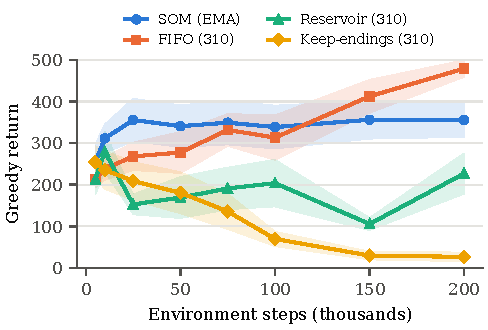
\includegraphics[width=\columnwidth]{figures/fig_curves.pdf}
\caption{Study 1: greedy return over training (mean over 10 seeds; band:
$\pm$1 standard error). All memories store about 3\,400 numbers.}
\label{fig:curves}
\end{figure}

\paragraph{Against real data.} \Cref{fig:curves} shows the learning curves.
The SOM reached 254 after 5k steps and 356 after 25k and stayed between 339
and 356 afterwards; FIFO of the same memory rose more slowly but kept
improving, to 412 at 150k and 479 at 200k. Over the whole run they tied
(333 vs.\ 317; $+15.8$ $[-28.8, +56.1]$, 7 of 10 seeds), so the second claim
failed. The SOM led at every checkpoint up to 100k and trailed from 150k on
(\cref{fig:gap}); late, FIFO led by 51.6 points ($[-111.1, +0.7]$). The SOM
beat reservoir ($+139.9$ $[+98.2, +181.5]$) and keep-endings ($+189.9$
$[+140.1, +240.0]$) in all 10 seeds and tied FIFO with 10\,000 transitions
($+35.7$ $[-11.1, +87.9]$). Keep-endings collapsed late (27 at 200k): once the
agent rarely fails, its slots hold old endings. The full-covariance SOM tied
FIFO with 810 transitions ($-29.9$ $[-65.3, +10.0]$) and beat reservoir
($+96.6$) and keep-endings ($+46.0$) of that memory.

\begin{figure}[t]
\centering
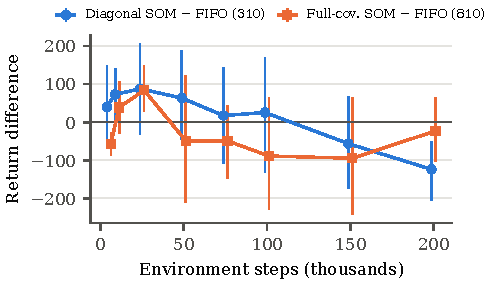
\includegraphics[width=\columnwidth]{figures/fig_gap.pdf}
\caption{Study 1: paired difference SOM minus FIFO of the same memory at each
checkpoint (95\% bootstrap intervals, 10 seeds; points offset horizontally).}
\label{fig:gap}
\end{figure}

\begin{figure}[t]
\centering
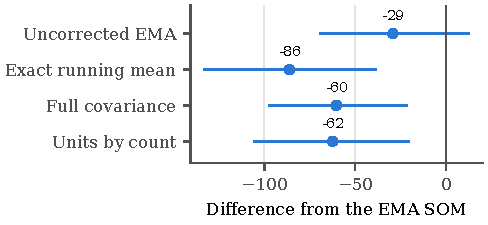
\includegraphics[width=\columnwidth]{figures/fig_ablation.pdf}
\caption{Study 1: whole-run score of each variant minus the EMA SOM (95\%
bootstrap intervals, 10 seeds).}
\label{fig:ablation}
\end{figure}

\paragraph{Variants.} \Cref{fig:ablation} compares each variant with the
reference. The uncorrected EMA did not differ detectably ($-29.2$ $[-70.2,
+12.4]$; first claim held), as expected, since at $\alpha = 0.9$ the
uncorrected bias is gone after two hits. The exact average lost 86.2 points
($[-133.9, -38.7]$), full covariances 60.3 ($[-97.6, -22.1]$) and choosing
units by their counts 62.4 ($[-106.3, -19.8]$). With full covariances, the
exact average lost to the EMA again ($-82.7$ $[-118.1, -38.3]$).

\paragraph{What the memories generate.} \Cref{tab:diag} reports the
generated data at the end of training. The exact-average memories generated
far fewer endings (1.0\% and 0.4\%) than the EMA memory (4.0\%). Every memory
used 98 to 100 of its 100 units and generated both actions about equally
often.

\begin{table}[t]
\caption{Study 1: generated transitions after 200k steps (5\,000 per run, mean
over seeds). CartPole's reward is always 1.}
\label{tab:diag}
\centering
\small
\begin{tabular}{lcc}
\toprule
SOM & Ending rate & Reward range \\
\midrule
EMA & 4.0\% & $[0.85, 1.16]$ \\
EMA, uncorrected & 4.6\% & $[0.74, 1.35]$ \\
Exact & 1.0\% & $[0.99, 1.01]$ \\
EMA, units by count & 3.0\% & $[0.99, 1.01]$ \\
Full cov., EMA & 2.9\% & $[0.37, 1.80]$ \\
Full cov., uncorrected & 4.9\% & $[0.49, 1.39]$ \\
Full cov., exact & 0.4\% & $[0.99, 1.01]$ \\
\bottomrule
\end{tabular}
\end{table}

\subsection{Study 2: averaging weight and ending decoding}
\label{sec:res-alpha}

Study 1 left two explanations for the exact average's deficit:
\emph{recency}, since the EMA follows each unit's latest transitions while
the exact average weights all of its history equally, and the \emph{ending
rate}, since the exact memories generated four to ten times fewer endings.
Study 2 varied the EMA weight $\alpha \in \{0.99, 0.9, 0.5, 0.1, 0.01\}$ and
the exact average, all with rounded endings, and ran the EMA ($\alpha =
0.9$) and exact memories also with Bernoulli endings. Claims stated before
the run: $\alpha = 0.9$ beats $\alpha = 0.01$ and the exact average; the SOM
does not lose to FIFO over the whole run and trails it late.

\begin{figure}[t]
\centering
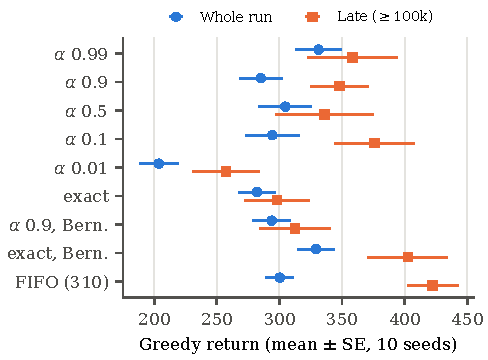
\includegraphics[width=\columnwidth]{figures/fig_alpha.pdf}
\caption{Study 2 (seeds 110--119): whole-run and late scores of every arm
(mean $\pm$ standard error, 10 seeds). ``Bern.'': Bernoulli endings.}
\label{fig:alpha}
\end{figure}

\begin{table}[t]
\caption{Study 2: key comparisons (paired difference, 95\% bootstrap
interval, seeds won of 10).}
\label{tab:alpha}
\centering
\small
\begin{tabular}{ll}
\toprule
Comparison & Difference \\
\midrule
\multicolumn{2}{l}{\emph{Whole-run score}} \\
$\alpha$ 0.9 $-$ $\alpha$ 0.01 & $+81.5$ $[+36.7, +127.5]$, 8 \\
$\alpha$ 0.9 $-$ exact & $+3.0$ $[-43.7, +45.2]$, 7 \\
$\alpha$ 0.9 $-$ FIFO (310) & $-15.1$ $[-40.7, +13.7]$, 3 \\
Exact, Bern.\ $-$ exact & $+47.2$ $[+21.4, +72.2]$, 9 \\
Exact, Bern.\ $-$ $\alpha$ 0.9, Bern. & $+35.5$ $[+12.7, +58.1]$, 9 \\
$\alpha$ 0.9, Bern.\ $-$ $\alpha$ 0.9 & $+8.7$ $[-26.1, +46.6]$, 4 \\
$\alpha$ 0.99 $-$ $\alpha$ 0.9 & $+46.1$ $[+12.0, +78.8]$, 7 \\
\midrule
\multicolumn{2}{l}{\emph{Late score}} \\
$\alpha$ 0.9 $-$ FIFO (310) & $-74.5$ $[-116.5, -25.3]$, 2 \\
Exact, Bern.\ $-$ exact & $+104.6$ $[+56.4, +152.0]$, 10 \\
Exact, Bern.\ $-$ FIFO (310) & $-19.8$ $[-108.1, +70.2]$, 6 \\
\bottomrule
\end{tabular}
\end{table}

\paragraph{Claims.} $\alpha = 0.9$ beat $\alpha = 0.01$ ($+81.5$) but not the
exact average ($+3.0$ $[-43.7, +45.2]$): the first claim held for one
comparison and failed for the other. The second claim held: the SOM tied
FIFO over the whole run and trailed it late ($-74.5$ $[-116.5, -25.3]$).

\paragraph{Ending decoding (exploratory).} Bernoulli endings changed the
exact memory the most: $+47.2$ over the whole run (9 of 10 seeds) and
$+104.6$ late (all 10 seeds), although its generated ending rate rose only
from 0.72\% to 1.02\%. It was then the best SOM memory over the whole run
(329), together with $\alpha = 0.99$ (331), and the only one that did not
trail FIFO late ($-19.8$ $[-108.1, +70.2]$). For the EMA memory, Bernoulli
endings changed little ($+8.7$).

\paragraph{The averaging weight.} Whole-run scores were 331, 285, 305, 294
and 204 for $\alpha$ = 0.99, 0.9, 0.5, 0.1 and 0.01, and 282 for the exact
average, which beat $\alpha = 0.01$ by 78.5 points ($[+29.9, +125.5]$). More
recency did not help steadily. The sweep is confounded at small $\alpha$:
because the EMA starts at zero, a unit's first variance is $\alpha x^2$,
which the correction scales to $x^2$ and which fades by a factor $1 - \alpha$
per hit. Slow averages keep this spread for longer; generated rewards (always
1 in the data) spread over $[0.43, 1.85]$ at $\alpha = 0.99$ but $[-1.73,
3.55]$ at $\alpha = 0.01$, while the exact average stays within $[0.99,
1.01]$.

\subsection{Study 3: replication}
\label{sec:res-repl}

Study 3 repeated the exact memory with Bernoulli endings on 20 new seeds,
against the same memory with rounded endings, the EMA memory ($\alpha =
0.9$, rounded) and FIFO of the same memory. Claims stated before the run:
(1) it beats the EMA memory over the whole run; (2) it beats its
rounded-ending version over the whole run and late; (3) it does not trail
FIFO late; (4) the EMA memory trails FIFO late.

\begin{figure}[t]
\centering
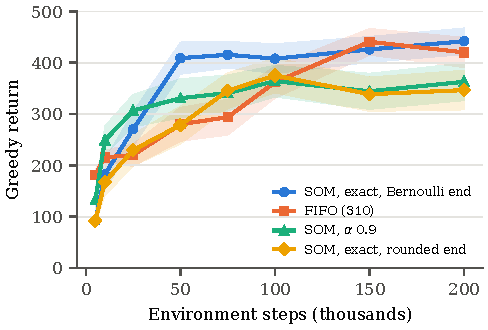
\includegraphics[width=\columnwidth]{figures/fig_replication.pdf}
\caption{Study 3 (seeds 120--139): greedy return over training (mean over 20
seeds; band: $\pm$1 standard error). All memories store about 3\,400
numbers.}
\label{fig:repl}
\end{figure}

\begin{table}[t]
\caption{Study 3 and pooled results. Paired difference, 95\% bootstrap
interval, seeds won. ``Exact+B'': exact average with Bernoulli endings;
``EMA'': $\alpha = 0.9$ with rounded endings.}
\label{tab:repl}
\centering
\small
\begin{tabular}{lll}
\toprule
Comparison & 20 seeds (Study 3) & 30 seeds (2 and 3) \\
\midrule
\multicolumn{3}{l}{\emph{Whole-run score}} \\
1.\ Exact+B $-$ EMA & $+26.7$ $[-3.5, +55.1]$, 13 & $+32.5$ $[+6.6, +58.8]$, 20 \\
2.\ Exact+B $-$ exact & $+58.8$ $[+23.7, +92.7]$, 14 & $+54.9$ $[+30.0, +79.3]$, 23 \\
\quad Exact+B $-$ FIFO & $+28.7$ $[+1.2, +56.1]$, 15 & $+28.8$ $[+7.7, +49.9]$, 23 \\
\midrule
\multicolumn{3}{l}{\emph{Late score ($\geq$100k)}} \\
\quad Exact+B $-$ EMA & $+68.1$ $[+16.4, +117.0]$, 16 & $+63.6$ $[+19.6, +106.8]$, 22 \\
2.\ Exact+B $-$ exact & $+71.7$ $[+25.1, +115.0]$, 15 & $+82.7$ $[+47.5, +115.8]$, 25 \\
3.\ Exact+B $-$ FIFO & $+17.6$ $[-22.0, +57.2]$, 9 & $+5.1$ $[-36.5, +44.6]$, 15 \\
4.\ EMA $-$ FIFO & $-50.5$ $[-86.0, -12.5]$, 5 & $-58.5$ $[-87.0, -28.6]$, 7 \\
\bottomrule
\end{tabular}
\end{table}

\paragraph{Claims.} \Cref{tab:repl} gives the results. The first claim
failed on the new seeds ($+26.7$ $[-3.5, +55.1]$), although the exact memory
with Bernoulli endings beat the EMA memory late ($+68.1$) and over the 30
seeds of Studies 2 and 3 ($+32.5$ $[+6.6, +58.8]$). The other three claims
held. Not named in the claims: it beat FIFO over the whole run ($+28.7$
$[+1.2, +56.1]$, 15 of 20 seeds).

\paragraph{Over training.} \Cref{fig:repl} shows a slow start, a clear lead
in the middle of training and a tie at the end. At 5k steps the exact memory
with Bernoulli endings was behind FIFO (91 vs.\ 182, 1 of 20 seeds); at 50k
it led by 129 points (409 vs.\ 280, $[+38, +213]$); at 200k the two were
level (442 vs.\ 420, $+22$ $[-37, +83]$). Its whole-run means in Studies 2 and
3 were 329 and 330.

\paragraph{Over all seeds.} Pooled over 40 seeds (100--139), the EMA memory
tied FIFO over the whole run ($+1.2$ $[-15.3, +17.6]$) and trailed it late
($-56.8$ $[-82.8, -29.6]$), and the exact memory with rounded endings lost to
both ($-38.4$ and $-37.2$).

\subsection{Study 4: burn-in and hybrid averaging}
\label{sec:res-burnin}

Study 4 asked whether the slow start of the exact memory with Bernoulli
endings can be removed. A diagnostic on development seeds pointed to two
candidates: units with few hits, which produced 23--38\% of generated
transitions at 1k steps but only 4--10\% at 5k; and averages that keep
transitions from where a unit used to be while the map still moves, since the
one-step physics error of the exact memory's generated transitions did not
fall over the first 25k steps. We compared the exact memory against burn-in
with $K = 5$ and $K = 20$, the hybrid average ($\kappa_{\min} = 0.01$), the
hybrid average with $K = 20$, and FIFO of the same memory, all with
Bernoulli endings, on 20 new seeds. Claims stated before the run: (1) burn-in
with $K = 20$ and (2) the hybrid average raise the early score; (3) neither
lowers the whole-run score.

\begin{figure}[t]
\centering
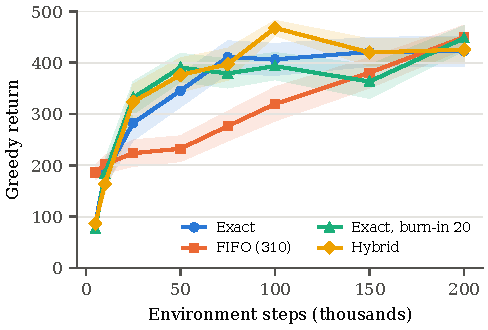
\includegraphics[width=\columnwidth]{figures/fig_burnin.pdf}
\caption{Study 4 (seeds 140--159): greedy return over training (mean over 20
seeds; band: $\pm$1 standard error). All SOM memories use Bernoulli endings;
all memories store about 3\,400 numbers.}
\label{fig:burnin}
\end{figure}

\begin{table}[t]
\caption{Study 4: claims and comparisons with FIFO (paired difference, 95\%
bootstrap interval, seeds won of 20). Early: mean of 5k, 10k and 25k.}
\label{tab:burnin}
\centering
\small
\begin{tabular}{ll}
\toprule
Comparison & Difference \\
\midrule
1.\ Burn-in 20 $-$ exact, early & $+13.1$ $[-12.8, +39.5]$, 12 \\
2.\ Hybrid $-$ exact, early & $+7.6$ $[-20.3, +33.8]$, 11 \\
3.\ Burn-in 20 $-$ exact, whole & $+0.9$ $[-25.2, +27.8]$, 9 \\
3.\ Hybrid $-$ exact, whole & $+12.9$ $[-18.4, +46.1]$, 10 \\
\quad Hybrid, burn-in 20 $-$ exact, early & $+30.0$ $[-3.2, +61.9]$, 14 \\
\midrule
\quad Exact $-$ FIFO, whole & $+35.9$ $[+3.7, +65.5]$, 16 \\
\quad Hybrid $-$ FIFO, whole & $+48.8$ $[+16.7, +77.8]$, 16 \\
\quad Hybrid $-$ FIFO, late & $+54.5$ $[+15.3, +95.7]$, 14 \\
\quad Exact $-$ FIFO at 5k & $-99.5$ $[-126.0, -75.0]$, 0 \\
\bottomrule
\end{tabular}
\end{table}

\paragraph{Claims.} Neither remedy raised the early score detectably:
$+13.1$ $[-12.8, +39.5]$ for burn-in with $K = 20$ and $+7.6$ $[-20.3,
+33.8]$ for the hybrid average, so claims 1 and 2 failed. Neither lowered the
whole-run score, so claim 3 held (\cref{tab:burnin}). Combining the two gave
the largest early gain ($+30.0$ $[-3.2, +61.9]$), also not detectable.

\paragraph{The first checkpoint.} At 5k steps every SOM memory scored 75 to
86 and FIFO 186; FIFO was ahead in 18 to 20 of 20 seeds for every SOM memory.
By 25k steps every SOM memory was ahead of FIFO on average (\cref{fig:burnin}). Neither
excluding units with few hits nor forgetting stale transitions changed the
first checkpoint, and the hybrid average is identical to the exact average
for a unit's first 100 hits, which covers most units at 5k steps. The EMA
memory ($\alpha = 0.9$) scored 132 to 254 at 5k steps in Studies 1--3, so
fast averaging helps at the very start, where exact and hybrid averages do
not.

\paragraph{Against FIFO (exploratory).} Every SOM memory in Study 4 beat FIFO
over the whole run (by 35.9 to 50.7 points, all intervals above 0), and the
hybrid memory also beat it late ($+54.5$ $[+15.3, +95.7]$). FIFO scored lower
in this study (284) than in Studies 1--3 (300--317). Pooled over Studies 2--4
(50 seeds), the exact memory with Bernoulli endings beat FIFO over the whole
run by $+31.6$ $[+13.7, +48.7]$ (39 of 50 seeds) and tied it late ($+16.4$
$[-15.5, +47.7]$); it was behind at 5k ($-87.8$, 3 of 50 seeds) and ahead at
25k ($+68.7$) and 50k ($+117.9$ $[+68.1, +167.8]$).

\subsection{Study 5: the averaging rate}
\label{sec:res-rate}

Studies 2--4 tested EMA rates other than 0.9 only with rounded endings and a
zero start. Study 5 compared, with Bernoulli endings and a clean start, the
hybrid average with floor rates 0.9, 0.5, 0.1, 0.03 and 0.01 (exact for a
unit's first $1/\text{rate}$ hits, an EMA with that weight afterwards), the
exact average, a schedule that uses rate 0.9 for the first 10\,000
transitions of the stream and exact averaging afterwards (``0.9, then
exact''), and FIFO of the same memory, on 20 new seeds. Claims stated before
the run: (1) rate 0.9 trails the exact average late; (2) rates 0.03 and 0.01
do not differ from it over the whole run; (3) ``0.9, then exact'' beats it at
5k steps and does not lose to it over the whole run.

\begin{figure}[t]
\centering
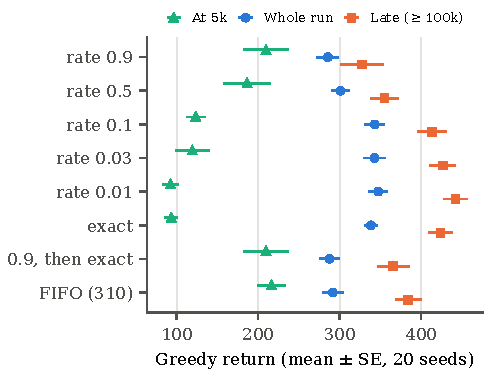
\includegraphics[width=\columnwidth]{figures/fig_rate.pdf}
\caption{Study 5 (seeds 160--179): score at 5k steps, whole-run and late
scores per averaging rate (mean $\pm$ standard error, 20 seeds). All SOM
memories use Bernoulli endings and a clean start.}
\label{fig:rate}
\end{figure}

\begin{table}[t]
\caption{Study 5: claims and comparisons with the exact average (paired
difference, 95\% bootstrap interval, seeds won of 20).}
\label{tab:rate}
\centering
\small
\begin{tabular}{ll}
\toprule
Comparison & Difference \\
\midrule
1.\ Rate 0.9 $-$ exact, late & $-96.2$ $[-148.7, -46.6]$, 5 \\
2.\ Rate 0.03 $-$ exact, whole & $+4.1$ $[-28.7, +37.4]$, 9 \\
2.\ Rate 0.01 $-$ exact, whole & $+8.9$ $[-20.4, +36.7]$, 12 \\
3.\ 0.9, then exact $-$ exact, 5k & $+116.2$ $[+61.3, +176.0]$, 18 \\
3.\ 0.9, then exact $-$ exact, whole & $-50.9$ $[-72.8, -28.9]$, 3 \\
\midrule
\quad Rate 0.5 $-$ exact, 5k & $+92.9$ $[+44.3, +148.2]$, 18 \\
\quad Rate 0.5 $-$ exact, late & $-68.5$ $[-112.0, -32.5]$, 2 \\
\quad Rate 0.1 $-$ exact, 5k & $+30.1$ $[+6.8, +54.4]$, 13 \\
\quad Rate 0.1 $-$ exact, whole & $+4.5$ $[-24.7, +34.0]$, 11 \\
\bottomrule
\end{tabular}
\end{table}

\paragraph{Claims.} Rate 0.9 trailed the exact average late by 96.2 points
(claim 1 held). Rates 0.03 and 0.01 did not differ from it over the whole run
(claim 2 held). ``0.9, then exact'' beat the exact average at 5k steps by
116.2 points (18 of 20 seeds) but lost to it over the whole run by 50.9
($[-72.8, -28.9]$), so claim 3 failed.

\paragraph{A trade-off between start and finish.} \Cref{fig:rate} shows a
single pattern. Fast rates (0.9, 0.5) scored about 185--210 at 5k steps, close to
FIFO (216), but trailed the exact average late by 69--96 points. Slow rates
(0.03, 0.01) behaved like the exact average: about 93--120 at 5k steps and
the best late scores (427--442). Rate 0.1 sat in between: higher than the
exact average at 5k ($+30.1$ $[+6.8, +54.4]$) with no detectable loss over
the whole run ($+4.5$) or late ($-10.2$ $[-44.8, +25.4]$).

\paragraph{Why the schedule failed (exploratory).} ``0.9, then exact''
dropped to 132 at 25k steps, below every other arm. At the switch the median
unit had about 100 hits (development check on recorded data), so afterwards
a new transition moves the unit's mean by about 1\%, while the mean itself
was, under rate 0.9, roughly the unit's last transition before the switch.
The schedule therefore froze each unit near one transition, including its
ending value. Restarting the exact average at the switch would avoid this;
we have not tested it.

\paragraph{Against FIFO (exploratory).} The exact average beat FIFO over the
whole run by 46.7 points ($[+18.9, +74.7]$, 18 of 20 seeds) and late by 39.5
($[+0.4, +80.3]$); rates 0.1, 0.03 and 0.01 also beat it over the whole run
(by 51--56). Pooled over Studies 2--5 (70 seeds), the exact average with
Bernoulli endings beat FIFO over the whole run by $+36.0$ $[+20.8, +50.9]$
(57 of 70 seeds) and late by $+23.0$ $[-2.6, +48.0]$, and trailed it only at
5k ($-97.8$, 3 of 70). Pooled over Studies 4--5 (40 seeds), the rate-0.01
hybrid beat FIFO over the whole run ($+52.2$ $[+29.2, +74.2]$) and late
($+56.3$ $[+29.0, +83.0]$) and did not differ detectably from the exact
average ($+10.9$ $[-10.1, +32.9]$).

\section{Discussion}
\label{sec:discussion}

\paragraph{Generating endings is the critical step.} In CartPole every step
earns the same reward, and only terminal transitions tell the agent which
states are dangerous. With rounded endings, a unit generates endings only if
its ending value is large or its spread is wide, so the units that generate
endings depend on their spread rather than on their recorded ending rate.
Bernoulli endings make every unit generate endings at its recorded rate.
This mattered most for exact averages, whose ending values are small, stable
rates: the change raised their late score by 105 points while their overall
ending rate rose by only about 40\%, which suggests that \emph{which} units
generate endings matters more than how many endings are generated. We have
not tested this directly.

\paragraph{Recency did not explain the differences.} With $\alpha = 0.9$ a
unit's mean is about 90\% its latest transition, so the EMA memory behaves
like ``the latest transition in each of 100 regions, plus noise''. This
reading suggested that recency explained its advantage over exact averages
in Study 1. Studies 2 and 3 do not support it: exact averages tied the EMA on
new seeds, and with Bernoulli endings they were best late in training, when
stale statistics should hurt most. The averaging-weight sweep was not
monotone either.

\paragraph{The late gap to FIFO.} The EMA memory trailed FIFO late in all
three studies (by 57 points over 40 seeds). The exact memory with Bernoulli
endings did not (30 seeds: $+5$ $[-37, +45]$), so the late gap is not a limit
of a memory that stores no transitions. A memory that weights each unit's
whole history equally matched one that holds only the most recent
transitions.

\paragraph{Start against finish.} The exact memory with Bernoulli endings
was behind FIFO at 5k steps in 67 of 70 seeds and ahead from 25k steps on.
Neither a burn-in threshold nor slow forgetting changed the first checkpoint
(Study 4); a fast averaging rate did (Study 5), at the cost of late
performance. A unit that follows its latest transitions helps while the map
and the policy change quickly; a unit that remembers its whole history helps
once there is more to remember. Rate 0.1 recovered part of the start without
a detectable loss later, and a schedule that restarts exact averaging at the
switch, rather than continuing from a fast average, remains to be tested.

\paragraph{Distance and covariance.} Full covariances make the sampled change
of state follow the sampled state and gave the smallest one-step physics
error on recorded data (0.0026 vs.\ 0.0037), yet they lost with the EMA,
whose covariance estimate rests on the last one or two transitions and is
noisy in 11 dimensions. Full covariances with exact averages and Bernoulli
endings remain untested.

\paragraph{The ending term of the distance.} On recorded data no unit's
ending weight rounded to 1, so the ending-mismatch term in
\cref{eq:distance} never distinguished units in a single online pass.
Endings shared units with other transitions and were generated through each
unit's ending statistic.

\paragraph{Limitations.} One task, one map size and one agent; 10 seeds in
Studies 1 and 2, 20 in Studies 3--5. Comparisons not named in a study's claims are
many and should be read as leads. Online DQN returns vary widely between
seeds (standard deviation of the whole-run score across seeds 25--75 in
Study 1), and the same arm's mean differed by up to 47 points between two
10-seed studies. The EMA's zero start leaves a spurious first variance that
lasts longer for small $\alpha$. The map's step size decays with the episode
index, so the map moves less as episodes lengthen.

\section{Conclusion}
\label{sec:conclusion}

A single SOM that stores no transitions can be the only replay memory of an
online DQN agent and match a FIFO buffer of real transitions with the same
memory. Across these studies, how each unit summarises its transitions and
generates episode endings mattered more than how transitions are assigned to
units. With exact per-unit averages and endings drawn at each unit's
recorded rate, the map beat FIFO over the whole run on CartPole (70 seeds).
The averaging rate trades the first few thousand steps against the end of
training: fast rates start like FIFO but fall behind later, slow rates and
exact averages start slowly but finish best. Next steps are schedules that
get both, other tasks and map sizes, and uncertainty-aware generation built
on this memory.

\bibliography{references}
\bibliographystyle{icml2026}

\newpage
\appendix
\onecolumn

\section{All Results}
\label{app:all}

\begin{table}[h]
\caption{Study 1 (seeds 100--109): mean greedy return at each checkpoint
(thousands of steps), whole-run and late scores, and the standard deviation
of the whole-run score across seeds.}
\label{tab:all}
\centering
\small
\begin{tabular}{lrrrrrrrrrrr}
\toprule
Arm & 5 & 10 & 25 & 50 & 75 & 100 & 150 & 200 & Whole & Late & SD \\
\midrule
\multicolumn{12}{l}{\emph{SOM, diagonal (3\,418 numbers)}} \\
EMA & 254 & 311 & 356 & 341 & 349 & 339 & 356 & 355 & 333 & 350 & 50 \\
EMA, uncorrected & 190 & 241 & 250 & 367 & 409 & 360 & 353 & 257 & 303 & 323 & 55 \\
Exact & 70 & 175 & 179 & 269 & 361 & 335 & 283 & 298 & 246 & 305 & 54 \\
EMA, units by count & 177 & 183 & 264 & 269 & 332 & 279 & 351 & 307 & 270 & 312 & 50 \\
\multicolumn{12}{l}{\emph{SOM, full covariance (8\,918 numbers)}} \\
EMA & 130 & 272 & 240 & 275 & 281 & 260 & 323 & 398 & 272 & 327 & 40 \\
EMA, uncorrected & 158 & 327 & 244 & 281 & 244 & 310 & 322 & 382 & 283 & 338 & 44 \\
Exact & 164 & 208 & 176 & 196 & 253 & 190 & 180 & 149 & 190 & 173 & 49 \\
\multicolumn{12}{l}{\emph{Real transitions, 310}} \\
FIFO & 214 & 238 & 268 & 277 & 332 & 313 & 412 & 479 & 317 & 402 & 44 \\
Reservoir & 213 & 279 & 153 & 169 & 191 & 204 & 106 & 227 & 193 & 179 & 39 \\
Keep-endings & 254 & 236 & 209 & 181 & 136 & 70 & 30 & 27 & 143 & 42 & 75 \\
\multicolumn{12}{l}{\emph{Real transitions, 810}} \\
FIFO & 188 & 233 & 156 & 324 & 330 & 348 & 418 & 421 & 302 & 396 & 49 \\
Reservoir & 198 & 191 & 162 & 172 & 187 & 186 & 168 & 144 & 176 & 166 & 25 \\
Keep-endings & 299 & 288 & 173 & 233 & 249 & 210 & 173 & 185 & 226 & 189 & 52 \\
\multicolumn{12}{l}{\emph{Real transitions, 10\,000 (reference)}} \\
FIFO & 207 & 175 & 166 & 279 & 428 & 423 & 322 & 374 & 297 & 373 & 52 \\
\bottomrule
\end{tabular}
\end{table}

\begin{table}[h]
\caption{Study 1: paired differences (mean, 95\% bootstrap interval over
seeds, seeds won of 10).}
\label{tab:pairs}
\centering
\small
\begin{tabular}{lll}
\toprule
Comparison & Whole run & Late ($\geq$100k) \\
\midrule
EMA uncorrected $-$ EMA & $-29.2$ $[-70.2, +12.4]$, 2 & $-26.6$ $[-100.7, +50.1]$, 3 \\
Exact $-$ EMA & $-86.2$ $[-133.9, -38.7]$, 2 & $-44.7$ $[-117.2, +35.2]$, 3 \\
Full $-$ diagonal (EMA) & $-60.3$ $[-97.6, -22.1]$, 1 & $-23.0$ $[-70.1, +30.6]$, 3 \\
Full: uncorrected $-$ EMA & $+11.1$ $[-35.0, +57.7]$, 6 & $+11.0$ $[-78.2, +101.7]$, 5 \\
Full: exact $-$ EMA & $-82.7$ $[-118.1, -38.3]$, 2 & $-153.9$ $[-225.7, -89.0]$, 0 \\
Units by count $-$ uniform & $-62.4$ $[-106.3, -19.8]$, 2 & $-37.8$ $[-121.8, +49.9]$, 5 \\
\midrule
EMA $-$ FIFO (310) & $+15.8$ $[-28.8, +56.1]$, 7 & $-51.6$ $[-111.1, +0.7]$, 4 \\
EMA $-$ reservoir (310) & $+139.9$ $[+98.2, +181.5]$, 10 & $+171.3$ $[+101.5, +242.2]$, 9 \\
EMA $-$ keep-endings (310) & $+189.9$ $[+140.1, +240.0]$, 10 & $+308.0$ $[+264.1, +353.2]$, 10 \\
EMA $-$ FIFO (10\,000) & $+35.7$ $[-11.1, +87.9]$, 6 & $-23.4$ $[-107.5, +77.6]$, 4 \\
Exact $-$ FIFO (310) & $-70.4$ $[-111.5, -26.6]$, 2 & $-96.3$ $[-162.1, -35.4]$, 1 \\
Full EMA $-$ FIFO (810) & $-29.9$ $[-65.3, +10.0]$, 3 & $-68.9$ $[-150.8, +16.0]$, 3 \\
Full EMA $-$ reservoir (810) & $+96.6$ $[+59.0, +130.8]$, 9 & $+161.4$ $[+73.1, +240.9]$, 8 \\
Full EMA $-$ keep-endings (810) & $+46.0$ $[+2.9, +92.2]$, 8 & $+137.6$ $[+65.9, +214.7]$, 9 \\
Full exact $-$ FIFO (810) & $-112.6$ $[-151.4, -72.4]$, 0 & $-222.8$ $[-290.0, -153.5]$, 0 \\
\bottomrule
\end{tabular}
\end{table}

\begin{table}[h]
\caption{Study 1: SOM minus FIFO at each checkpoint (mean, 95\% interval,
seeds won of 10).}
\label{tab:gap}
\centering
\small
\begin{tabular}{rlll}
\toprule
Steps & Diagonal EMA $-$ FIFO (310) & Full EMA $-$ FIFO (810) & Diagonal EMA $-$ FIFO (10\,000) \\
\midrule
5k & $+39.9$ $[-67.5, +147.8]$, 5 & $-57.3$ $[-88.6, -26.0]$, 1 & $+46.6$ $[-35.7, +137.0]$, 5 \\
10k & $+73.0$ $[+1.6, +141.3]$, 7 & $+38.9$ $[-29.1, +105.9]$, 7 & $+136.1$ $[+77.2, +195.0]$, 9 \\
25k & $+87.5$ $[-32.8, +206.6]$, 6 & $+83.8$ $[+29.2, +151.8]$, 9 & $+190.0$ $[+94.0, +287.1]$, 9 \\
50k & $+63.4$ $[-46.7, +186.7]$, 4 & $-49.0$ $[-209.3, +124.2]$, 3 & $+61.7$ $[-99.2, +205.7]$, 6 \\
75k & $+17.4$ $[-106.0, +142.4]$, 4 & $-49.0$ $[-148.3, +46.5]$, 3 & $-78.9$ $[-194.9, +32.3]$, 3 \\
100k & $+25.4$ $[-130.6, +169.6]$, 6 & $-88.8$ $[-232.2, +60.1]$, 4 & $-84.8$ $[-222.8, +62.3]$, 2 \\
150k & $-56.3$ $[-176.4, +64.8]$, 3 & $-94.8$ $[-243.8, +67.3]$, 3 & $+33.6$ $[-137.7, +202.2]$, 5 \\
200k & $-123.8$ $[-201.6, -50.6]$, 0 & $-23.0$ $[-102.5, +63.5]$, 1 & $-18.9$ $[-131.0, +102.4]$, 3 \\
\bottomrule
\end{tabular}
\end{table}

\begin{table}[h]
\caption{Study 2 (seeds 110--119): mean greedy return per checkpoint,
whole-run and late scores, seed SD, and the generated ending rate at 200k
steps. All SOMs: diagonal, bias-corrected EMA or exact average, uniform
units.}
\label{tab:alpha-all}
\centering
\small
\begin{tabular}{lrrrrrrrrrrrr}
\toprule
Arm & 5 & 10 & 25 & 50 & 75 & 100 & 150 & 200 & Whole & Late & SD & Endings \\
\midrule
$\alpha$ 0.99 & 218 & 280 & 325 & 363 & 389 & 322 & 378 & 376 & 331 & 358 & 57 & 4.5\% \\
$\alpha$ 0.9 & 212 & 283 & 269 & 163 & 311 & 276 & 338 & 430 & 285 & 348 & 54 & 3.5\% \\
$\alpha$ 0.5 & 240 & 298 & 252 & 378 & 261 & 347 & 339 & 323 & 305 & 336 & 67 & 4.5\% \\
$\alpha$ 0.1 & 86 & 243 & 256 & 311 & 332 & 338 & 402 & 388 & 294 & 376 & 68 & 1.9\% \\
$\alpha$ 0.01 & 47 & 143 & 169 & 240 & 258 & 198 & 315 & 259 & 204 & 257 & 50 & 2.2\% \\
Exact & 96 & 238 & 287 & 411 & 331 & 384 & 319 & 191 & 282 & 298 & 47 & 0.7\% \\
$\alpha$ 0.9, Bernoulli & 183 & 319 & 257 & 290 & 365 & 278 & 303 & 357 & 294 & 313 & 47 & 5.7\% \\
Exact, Bernoulli & 112 & 229 & 334 & 364 & 389 & 353 & 398 & 457 & 329 & 403 & 47 & 1.0\% \\
FIFO (310) & 171 & 204 & 209 & 259 & 293 & 355 & 420 & 492 & 300 & 422 & 36 & -- \\
\bottomrule
\end{tabular}
\end{table}

\begin{table}[h]
\caption{Study 3 (seeds 120--139): mean greedy return per checkpoint,
whole-run and late scores, seed SD and generated ending rate at 200k steps.}
\label{tab:repl-all}
\centering
\small
\begin{tabular}{lrrrrrrrrrrrr}
\toprule
Arm & 5 & 10 & 25 & 50 & 75 & 100 & 150 & 200 & Whole & Late & SD & Endings \\
\midrule
Exact, Bernoulli & 91 & 182 & 270 & 409 & 415 & 408 & 426 & 442 & 330 & 425 & 53 & 1.1\% \\
Exact, rounded & 92 & 167 & 230 & 278 & 345 & 375 & 339 & 347 & 272 & 353 & 56 & 0.7\% \\
EMA ($\alpha$ 0.9), rounded & 132 & 249 & 307 & 331 & 341 & 364 & 344 & 363 & 304 & 357 & 45 & 4.6\% \\
FIFO (310) & 182 & 216 & 220 & 280 & 294 & 362 & 441 & 420 & 302 & 408 & 46 & -- \\
\bottomrule
\end{tabular}
\end{table}

\begin{table}[h]
\caption{Study 4 (seeds 140--159): mean greedy return per checkpoint, early,
whole-run and late scores, seed SD and generated ending rate at 200k steps.
All SOM memories: diagonal, Bernoulli endings, uniform choice among eligible
units.}
\label{tab:burnin-all}
\centering
\small
\begin{tabular}{lrrrrrrrrrrrrr}
\toprule
Arm & 5 & 10 & 25 & 50 & 75 & 100 & 150 & 200 & Early & Whole & Late & SD & Endings \\
\midrule
Exact & 86 & 182 & 282 & 345 & 411 & 406 & 421 & 422 & 184 & 320 & 417 & 61 & 1.2\% \\
Exact, burn-in 5 & 86 & 232 & 287 & 403 & 345 & 387 & 396 & 433 & 202 & 321 & 405 & 56 & 0.9\% \\
Exact, burn-in 20 & 76 & 183 & 331 & 390 & 379 & 393 & 363 & 448 & 197 & 320 & 401 & 49 & 1.0\% \\
Hybrid & 86 & 164 & 324 & 376 & 397 & 468 & 420 & 425 & 191 & 332 & 438 & 46 & 1.2\% \\
Hybrid, burn-in 20 & 75 & 192 & 374 & 391 & 374 & 415 & 417 & 438 & 214 & 334 & 423 & 57 & 1.1\% \\
FIFO (310) & 186 & 202 & 224 & 232 & 276 & 319 & 380 & 450 & 204 & 284 & 383 & 37 & -- \\
\bottomrule
\end{tabular}
\end{table}

\begin{table}[h]
\caption{Study 5 (seeds 160--179): mean greedy return per checkpoint, early,
whole-run and late scores, seed SD and generated ending rate at 200k steps.
All SOM memories: diagonal, Bernoulli endings, clean start.}
\label{tab:rate-all}
\centering
\small
\begin{tabular}{lrrrrrrrrrrrrr}
\toprule
Arm & 5 & 10 & 25 & 50 & 75 & 100 & 150 & 200 & Early & Whole & Late & SD & Endings \\
\midrule
Rate 0.9 & 210 & 260 & 258 & 245 & 331 & 283 & 330 & 369 & 242 & 286 & 328 & 60 & 4.7\% \\
Rate 0.5 & 187 & 295 & 242 & 296 & 324 & 368 & 367 & 330 & 241 & 301 & 355 & 50 & 3.9\% \\
Rate 0.1 & 124 & 271 & 325 & 404 & 380 & 391 & 413 & 437 & 240 & 343 & 413 & 56 & 1.3\% \\
Rate 0.03 & 119 & 268 & 299 & 362 & 413 & 422 & 441 & 417 & 229 & 343 & 427 & 59 & 1.2\% \\
Rate 0.01 & 93 & 220 & 327 & 412 & 401 & 431 & 458 & 438 & 213 & 347 & 442 & 52 & 1.1\% \\
Exact & 94 & 234 & 317 & 363 & 429 & 395 & 467 & 409 & 215 & 338 & 424 & 37 & 1.1\% \\
0.9, then exact & 210 & 260 & 132 & 278 & 324 & 336 & 390 & 371 & 200 & 288 & 366 & 57 & 1.7\% \\
FIFO (310) & 216 & 188 & 264 & 218 & 296 & 316 & 406 & 430 & 223 & 292 & 384 & 56 & -- \\
\bottomrule
\end{tabular}
\end{table}

\section{Implementation Details}
\label{app:impl}

The memory is \texttt{structured\_som.StructuredSOMBuffer}; the real buffers
are \texttt{replay\_buffers.RealBuffer}. Each run took 3--7 minutes on one
CPU core (Intel Core i7-14700F; Python 3.12.3, PyTorch 2.15.0, Gymnasium
1.4.0, NumPy 2.5.4). Every command, seed and script hash is listed in
\texttt{REPRODUCIBILITY.md}.

\paragraph{Checks before Study 1} (development seed 997, and the first
10\,000 transitions of a 60\,000-step random-policy CartPole dataset): every
memory ran for 6\,000 steps without error; with one hit, the bias-corrected
mean equals the transition; every unit held a single action; generated
ending rates were 3--5\% against 4.6\% in the data; the one-step physics
error of generated transitions was 0.0026--0.0053 (full covariance lowest);
and no terminal transition landed in a unit whose ending weight rounds to 1.

\end{document}
